% !TeX program = tectonic
\documentclass{beamer}
\usepackage[utf8]{inputenc}
\usepackage[T1]{fontenc}
\usepackage{lmodern}
\usepackage{amsmath, amssymb}
\usepackage{graphicx}
\usepackage{tikz}
\usetikzlibrary{arrows.meta,positioning,calc}
% Ensure figures auto-fit within slides by default
\setkeys{Gin}{width=\linewidth,height=0.62\textheight,keepaspectratio}
\usepackage{booktabs}
\usepackage{arydshln} % dashed lines in tables
\usepackage{array}    % advanced column types (m{...} for vertical centering)
\usepackage{hyperref}
\hypersetup{unicode=true}
% Sanitize PDF bookmarks: replace math/special macros with plain-text fallbacks
\pdfstringdefDisableCommands{%
  \def\textemdash{-}%
  \def\P{P}%
  \def\E{E}%
  \def\Var{Var}%
  \def\1{1}%
  \def\mathbb#1{#1}%
  \def\mathcal#1{#1}%
  \def\bm#1{#1}%
}
\usepackage{bm}
\usepackage{centernot} % for crossed implication symbols like \centernot\Rightarrow

% Notation and helpers
\newcommand{\R}{\mathbb{R}}
\renewcommand{\P}{\mathbb{P}}
\newcommand{\E}{\mathbb{E}}
\newcommand{\Var}{\operatorname{Var}}
\newcommand{\1}{\mathbf{1}}
\newcommand{\indep}{\perp\!\!\!\perp}
\newcommand{\toP}{\xrightarrow{\,\mathsf{P}\,}}
\newcommand{\toas}{\xrightarrow{\,\mathsf{a.s.}\,}}
\newcommand{\tod}{\xrightarrow{\,\mathcal{D}\,}}

% Helper for robust top-line commands
\newcommand{\robustcmd}[1]{\csname #1\endcsname}
% Provide a safe wrapper for text-formatting commands that may appear at line start
% Use \robustcmd{textbf}{...} where editors can strip a leading backslash accidentally.
\providecommand{\textbf}[1]{\robustcmd{textbf}{#1}}

\usetheme{Madrid}
\usecolortheme{default}
\setbeamertemplate{navigation symbols}{}

% Show a mini table of contents at the beginning of each section
\AtBeginSection[]{
  \begin{frame}{Outline}
    \robustcmd{tableofcontents}[currentsection,hideothersubsections]
  \end{frame}
}

\robustcmd{title}{Lesson 1 --- Statistical Modeling}
\robustcmd{subtitle}{Random Variables, Distributions, LLN, CLT}
\robustcmd{author}{Applied Statistics Course}
\robustcmd{date}{\today}

\begin{document}

\begin{frame}
  \robustcmd{titlepage}
\end{frame}

\section{Modeling Motivation}

% New: Modeling with Events \textemdash{} motivating examples
\begin{frame}{Why Probability? From Questions to Models}
  \textbf{Natural language} \,$\to$\, \textbf{mathematical model} via events and random variables.
  \begin{itemize}
    \item Web A/B test: "Is variant B better than A?" $\Rightarrow$ Encode clicks as Bernoulli trials; compare $p_A$ vs $p_B$.
    \item Manufacturing: "Are defects random and rare?" $\Rightarrow$ Model counts with Poisson; check fit.
  \end{itemize}
  \medskip
  \begin{block}{Language of sets and probability}
    Events are sets (subsets of $\Omega$). Questions like "did a click occur?" or "defects $\le 3$" translate to $A\in\mathcal{F}$ and $\P(A)$.
  \end{block}
  \textbf{Probability theory} provides mathematical tools designed to \textbf{formalize uncertainty} and enable rigorous \textbf{reasoning about random phenomena}.
\end{frame}

\begin{frame}{From Natural Language to Events and RVs}{}
  {\small
    \centering
    % Increase row height for readability
    \renewcommand{\arraystretch}{1.30}%
    \setlength{\dashlinedash}{1pt}\setlength{\dashlinegap}{1.5pt}% dashed pattern
    \begin{tabular}{@{}m{0.32\textwidth} m{0.30\textwidth} m{0.32\textwidth}@{}}
      \toprule
      \textbf{Natural question} & \textbf{Event / RV} & \textbf{Typical model} \\
      \midrule
      "Roll of a fair die?" & \shortstack[l]{$X\in\{1,\dots,6\}$,\\ event $E=\{X\text{ even}\}$} & \shortstack[l]{$X$ uniform on $\{1,\dots,6\}$;\\ $\P(X=k)=1/6$} \\
      \addlinespace[3pt]
      \cdashline{1-3}
      \addlinespace[3pt]
      "User clicks?" & \shortstack[l]{$C=\{\text{click}\}$,\\ indicator $X=\1_C$} & \shortstack[l]{$X\sim\mathrm{Bernoulli}(p)$;\\ compare $p_A$ vs $p_B$} \\
      \addlinespace[3pt]
      \cdashline{1-3}
      \addlinespace[3pt]
      "Defects in a batch?" & Count $D\in\{0,1,2,\dots\}$ & \shortstack[l]{$D\sim\mathrm{Poisson}(\lambda)$\\ (rare, independent)} \\
      \addlinespace[3pt]
      \cdashline{1-3}
      \addlinespace[3pt]
      "Time until failure?" & Continuous $T\ge 0$ & \shortstack[l]{$T\sim\mathrm{Exponential}(\lambda)$\\ (memoryless)} \\
      \bottomrule
  \end{tabular}}
  \bigskip

  {
    \centering
    \small
    \begin{minipage}{0.9\linewidth}
      \centering
      \textbf{Set operations encode logic:}\\ \alert{$A\cup B$} = "A or B",\enspace \alert{$A\cap B$} = "A and B"\\
      \alert{$A^c$} = "not A"
    \end{minipage}
  }
\end{frame}

\begin{frame}{Example: A/B Test as Bernoulli/Binomial}
  Each impression is a trial: click = 1, no click = 0. Variant-level CTR estimates $\hat p = \frac{\text{clicks}}{\text{impressions}}$.
  \begin{center}
    \includegraphics{figures/ab_test_ctr.png}
  \end{center}
  {\small Confidence intervals visualize uncertainty from finite samples.}
\end{frame}

\begin{frame}{Catchy: The Birthday Paradox}
  In a class of $n$ students, what's the chance at least two share a birthday? Surprisingly, at $n=23$ it's about 0.5.
  \begin{center}
    \includegraphics{figures/birthday_paradox.png}
  \end{center}
  {\small Shows how multiplicative complements and event counting yield unintuitive results.}
\end{frame}

\begin{frame}{Catchy: Monty Hall \textemdash{} Switch or Stay?}
  Game show setup: switching doors wins with probability $\approx 2/3$; simulation confirms the model.
  \begin{center}
    \includegraphics{figures/monty_hall.png}
  \end{center}
  {\small Encodes information and conditional probability; a great motivator for Bayes' rule.}
\end{frame}

\begin{frame}{Example: Defects as Poisson Counts}
  When events are rare and independent, counts in a fixed window often follow Poisson($\lambda$). Compare empirical distribution vs Poisson model.
  \begin{center}
    \includegraphics{figures/defects_poisson_by_batch.png}
  \end{center}
  {\small If the fit is reasonable, $\lambda$ summarizes the average defects per batch, guiding quality control.}
\end{frame}

\begin{frame}{Example: Time-to-Failure as Exponential}
  Waiting times between independent events are often modeled as Exponential($\lambda$). The survival is $S(t)=\P(T>t)=e^{-\lambda t}$.
  \begin{center}
    \includegraphics{figures/time_to_failure.png}
  \end{center}
  {\small Useful for reliability, queueing, and risk modeling.}
\end{frame}

\begin{frame}{Learning Objectives}
  \begin{itemize}
      \setlength{\itemsep}{0.45em}
    \item \textbf{Define random variables (RVs) and distributions}.\\[-0.25em]{\footnotesize Purpose: Map real-world uncertainty to mathematical objects and clarify what a distribution encodes.}
    \item \textbf{Use PMF/PDF/CDF to compute probabilities/quantiles}.\\[-0.25em]{\footnotesize Purpose: Turn event and threshold questions into computations to answer ``how likely?'' and ``what cutoff?''.}
    \item \textbf{Compute expectation, variance, and interpret moments}.\\[-0.25em]{\footnotesize Purpose: Summarize center and variability to compare models and quantify uncertainty/risk.}
    \item \textbf{Understand LLN and CLT (intuition + statements)}.\\[-0.25em]{\footnotesize Purpose: Explain why averages stabilize and when normal approximations apply, enabling CIs and tests.}
    \item \textbf{Connect descriptive statistics to probabilistic modeling}.\\[-0.25em]{\footnotesize Purpose: Bridge EDA to formal models so assumptions are explicit and limits understood.}
  \end{itemize}
\end{frame}

\section{Foundations and Random Variables}

\begin{frame}{Probability Space -- Recap}
  \textbf{Definition.} A probability space is a triple $(\Omega,\,\mathcal{F},\,\P)$ where:
  \begin{itemize}
    \item $\Omega$ is the sample space; $\mathcal{F}\subseteq 2^{\Omega}$ is a $\sigma$-algebra;
    \item $\P:\mathcal{F}\to[0,1]$ is a probability measure, $\P(\Omega)=1$, and $\P$ is countably additive.
  \end{itemize}
  \medskip
  \begin{block}{Basic properties for events $A,B\in\mathcal{F}$}
    \begin{itemize}
        \setlength{\itemsep}{0.25em}
      \item Bounds: $0\le \P(A)\le 1$, with $\P(\varnothing)=0$ and $\P(\Omega)=1$.
      \item Complement: $\P(A^c)=1-\P(A)$.
      \item Monotonicity: $A\subseteq B\;\Rightarrow\; \P(A)\le \P(B)$.
      \item Union/intersection: $\P(A\cup B)=\P(A)+\P(B)-\P(A\cap B)$.
      \item Disjoint additivity: if $A\cap B=\varnothing$, then $\P(A\cup B)=\P(A)+\P(B)$; extends to countable disjoint unions.
    \end{itemize}
  \end{block}
  {\small Events are the measurable statements about outcomes: elements of $\mathcal{F}$.}
\end{frame}

\begin{frame}{Random Variables and Laws}{}
  \begin{block}{Random variable}
    A map $X$ is \textbf{measurable} if for every Borel set $B\in\mathcal{B}(\R)$, the preimage $X^{-1}(B)=\{\omega\in\Omega:X(\omega)\in B\}\in\mathcal{F}$.\\[0.5em]

    A \textbf{real-valued random variable} is a measurable map $X:(\Omega,\mathcal{F})\to(\R,\mathcal{B}(\R))$.
  \end{block}

  \begin{block}{Law (distribution)}
    For $B\in\mathcal{B}(\R)$, the law of $X$ is the pushforward measure
    {\scriptsize\[
        \mu_X(B)=\P(X\in B)=\P\big(X^{-1}(B)\big).
    \]}
  \end{block}

  \begin{block}{Types of laws}
    Discrete (countable support; PMF $p_X$), absolutely continuous (PDF $f_X$; $F'_X=f_X$ a.e.), and mixed.
  \end{block}
\end{frame}

\begin{frame}{Why Random Variables are Useful?}
  \textbf{Same information, but easier to use:}
  \begin{itemize}
    \item A random variable $X:\Omega \to \mathbb{R}$ induces a distribution $\mathbb{P}_X$.
    \item Working with $X$ or $\mathbb{P}_X$ encodes the same probabilistic information.
    \item $\Rightarrow$ Random variables let us write \emph{equations} instead of handling sets and events.
  \end{itemize}

  \medskip
  \textbf{Advantages of random variables:}
  \begin{itemize}
    \item \textit{Algebraic manipulation:} can form $Y=2X+3$, $Z=X+Y$, etc.
    \item \textit{Compounding:} joint r.v.s describe multiple processes easily.
    \item \textit{Analytical tools:} enable expectations, variances, mgfs, characteristic functions.
    \item \textit{Modeling:} regression, Bayesian models, stochastic processes all rely on r.v.s.
  \end{itemize}

  \medskip
  \textbf{Key message:}
  Random variables = distributions in disguise, but far more convenient for \emph{calculation, composition, and modeling}.
\end{frame}

\begin{frame}{Discrete random variables: PMF}{}
  \begin{block}{What is a discrete RV?}
    $X$ takes values in a countable set $A=\{x_1,x_2,\dots\}$. Probability mass sits on points; probabilities \emph{add up} across values.
  \end{block}
  \vspace{-0.4em}
  \begin{block}{PMF (probability mass function)}
    The PMF $p_X(x)=\P(X=x)$ assigns a weight to each $x\in A$ with $p_X(x)\ge 0$ and $\sum_{x\in A} p_X(x)=1$. For any measurable $B$,
    {\scriptsize\[
        \P(X\in B)=\sum_{x\in A\cap B} p_X(x).
    \]}
    Interpretation: $p_X$ is a table (or bar chart) of \emph{weights} at allowed values.
  \end{block}
  Examples: Bernoulli$(p)$: $p(1)=p$, $p(0)=1-p$.\quad Poisson$(\lambda)$: $p(k)=e^{-\lambda}\,\lambda^k/k!$, $k=0,1,2,\dots$.
\end{frame}

\begin{frame}{Discrete random variables: CDF}{}
  {\small
    \begin{block}{CDF (cumulative distribution function)}
      $F_X(x)=\P(X\le x)$ accumulates mass up to $x$. For discrete $X$, $F_X$ is a non-decreasing \emph{step} function; at each support point $x$ the jump size equals $p_X(x)$. Between support points $F_X$ is flat.
    \end{block}
    \vspace{-0.4em}
    \begin{exampleblock}{Using the CDF}
      For $a<b$,
      {\scriptsize\[
          \P(a< X\le b)=F_X(b)-F_X(a),\qquad \P(X=x)=F_X(x)-F_X(x^-)=p_X(x).
      \]}
      Properties: non-decreasing, right-continuous, $\lim_{x\to-\infty}F_X=0$, $\lim_{x\to\infty}F_X=1$.
    \end{exampleblock}
    \vspace{-0.45em}
    \begin{alertblock}{When is the CDF meaningful?}
      A CDF requires a meaningful order on the support. For nominal categories (unordered), prefer category probabilities (PMF); only define cumulative quantities once an inherent or agreed ordinal scale exists.
    \end{alertblock}
  }
\end{frame}

% CDF meaningful vs not: pedagogical contrast
\begin{frame}{When the CDF \emph{does} make sense (ordered counts)}
  % Ordered discrete support example: Poisson-like defect counts
  \small
  \begin{columns}[T,totalwidth=\textwidth]
    \begin{column}{0.47\textwidth}
      \robustcmd{textbf}{PMF (Defect count)}\\[0.15em]
      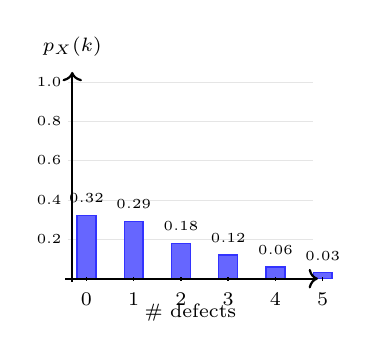
\begin{tikzpicture}[
        x=0.6cm,y=2.5cm,
        baseline=(current bounding box.north),
        every node/.style={font=\scriptsize}
      ]
        % Light grid for better readability
        \foreach \y in {0.2,0.4,0.6,0.8,1.0} {
          \draw[gray!20,very thin] (-0.1,\y) -- (5.1,\y);
        }
        % Example probabilities (sum to 1 roughly)
        \foreach [count=\k] \p in {0.32,0.29,0.18,0.12,0.06,0.03} {
           \pgfmathparse{\k-1}\let\x=\pgfmathresult
           \draw[fill=blue!60,draw=blue!80,line width=0.5pt] (\x+0.1,0) rectangle +(0.4,\p);
           \node[font=\tiny,anchor=south] at (\x+0.3,\p+0.015) {\pgfmathprintnumber[fixed,precision=2]{\p}};
        }
        % Professional axes with improved positioning
        \draw[->,line width=0.8pt] (-0.15,0) -- (5.2,0);
        \draw[->,line width=0.8pt] (0,-0.015) -- (0,1.05);
        % Y-axis label positioned above
        \node[font=\scriptsize,anchor=south] at (0,1.08) {$p_X(k)$};
        % X-axis label
        \node[font=\scriptsize,anchor=north] at (2.5,-0.08) {\# defects};
        % Improved axis ticks and labels
        \foreach \k in {0,...,5} {
          \draw[line width=0.5pt] (\k+0.3,-0.01) -- (\k+0.3,0.01);
          \node[font=\scriptsize,anchor=north] at (\k+0.3,-0.025) {\k};
        }
        \foreach \y in {0.2,0.4,0.6,0.8,1.0} {
          \draw[line width=0.5pt] (-0.02,\y) -- (0,\y);
          \node[font=\tiny,anchor=east] at (-0.025,\y) {\y};
        }
      \end{tikzpicture}

      \vspace{0.05em}
      \begin{block}{Natural ordering}
        Values $0 < 1 < 2 < \dots$ have clear meaning.\\
        Events like $\{X \le 2\}$ are interpretable.
      \end{block}
    \end{column}
    \begin{column}{0.47\textwidth}
      \robustcmd{textbf}{CDF (cumulative steps)}\\[0.15em]
      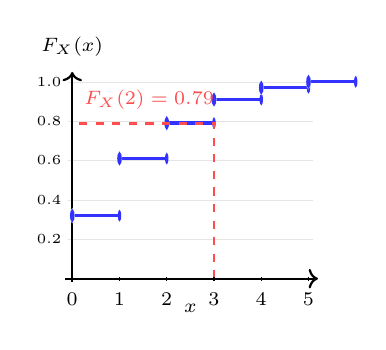
\begin{tikzpicture}[
        x=0.6cm,y=2.5cm,
        baseline=(current bounding box.north),
        every node/.style={font=\scriptsize}
      ]
        % Light grid for reference
        \foreach \y in {0.2,0.4,0.6,0.8,1.0} {
          \draw[gray!20,very thin] (-0.1,\y) -- (5.1,\y);
        }
        % Professional axes with improved positioning
        \draw[->,line width=0.8pt] (-0.15,0) -- (5.2,0);
        \draw[->,line width=0.8pt] (0,-0.015) -- (0,1.05);
        % Y-axis label positioned above
        \node[font=\scriptsize,anchor=south] at (0,1.08) {$F_X(x)$};
        % X-axis label
        \node[font=\scriptsize,anchor=north] at (2.5,-0.08) {$x$};
        % Steps with professional styling
        \foreach [count=\k] \f in {0.32,0.61,0.79,0.91,0.97,1.00} {
          \pgfmathparse{\k-1}\let\x=\pgfmathresult
          % horizontal step
          \draw[thick,blue!80,line width=1.2pt] (\x,\f) -- (\x+1,\f);
          % right endpoint (closed)
          \filldraw[blue!80] (\x+1,\f) circle (0.025);
          % left endpoint (open)
          \draw[thick,white,line width=1pt] (\x,\f) circle (0.025);
          \draw[thick,blue!80,line width=0.8pt] (\x,\f) circle (0.025);
        }
        % Highlight example: P(X ≤ 2) with better styling
        \draw[dashed,red!70,line width=1pt] (3,0) -- (3,0.79) -- (0,0.79);
        \node[font=\scriptsize,red!70,anchor=south west] at (0.05,0.81) {$F_X(2) = 0.79$};
        % Improved axis ticks and labels
        \foreach \k in {0,...,5} {
          \draw[line width=0.5pt] (\k,-0.01) -- (\k,0.01);
          \node[font=\scriptsize,anchor=north] at (\k,-0.025) {\k};
        }
        \foreach \y in {0.2,0.4,0.6,0.8,1.0} {
          \draw[line width=0.5pt] (-0.02,\y) -- (0,\y);
          \node[font=\tiny,anchor=east] at (-0.025,\y) {\y};
        }
      \end{tikzpicture}

      \vspace{0.05em}
      \begin{block}{Meaningful cumulation}
        $F_X(k) = \P(X \le k)$ answers\\
        concrete questions about defects.
      \end{block}
    \end{column}
  \end{columns}

  \vspace{0.05em}
  \begin{center}
    \alert{\large Key insight:} Natural ordering $\Rightarrow$ meaningful cumulative probabilities
  \end{center}
\end{frame}

\begin{frame}{When CDF is \emph{meaningless} (nominal categories)}
  \small
  \begin{columns}[T,totalwidth=\textwidth]
    \begin{column}{0.47\textwidth}
      \textbf{PMF for M\&M colors}\\[0.15em]
      \centering
      \includegraphics[width=\textwidth,height=0.35\textheight,keepaspectratio]{figures/mm_pmf.png}

      \vspace{0.5em}
      \begin{block}{No natural order}
        Colors are \emph{nominal categories}.\\
        No meaningful $<$ relationship exists.
      \end{block}
    \end{column}
    \begin{column}{0.47\textwidth}
      \textbf{Arbitrary "CDF" (alphabetical)}\\[0.15em]
      \centering
      \includegraphics[width=\textwidth,height=0.35\textheight,keepaspectratio]{figures/mm_cdf.png}

      \begin{alertblock}{Why this fails}
        Different orderings give different "CDFs".\\
        $\P(\text{color} \le \text{Green})$ is nonsense!
      \end{alertblock}
    \end{column}
  \end{columns}
  \vspace{0.05em}
  \begin{center}
    \alert{\large Key insight:} No natural order $\Rightarrow$ CDF is arbitrary and meaningless
  \end{center}
\end{frame}

\begin{frame}{Continuous random variables: PDF}{}
  \begin{block}{What is a continuous RV?}
    No atoms: $\P(X=a)=0$ for every $a\in\R$. Probabilities live on intervals/sets, not single points.
  \end{block}

  \begin{block}{PDF (probability density function)}
    A nonnegative function $f_X$ with $\int_{\R} f_X(x)\,dx=1$ such that for any measurable $B$, $\P(X\in B)=\int_B f_X(x)\,dx$. For $a<b$,
    {\scriptsize\[
        \P(a< X\le b)=\int_a^b f_X(x)\,dx.
    \]}
    Intuition: $f_X$ is a \emph{height}; probability is \emph{area under the curve}. The PDF itself is not a probability.
  \end{block}

  \textbf{Examples:} Uniform$(a,b)$: $f=1/(b-a)$ on $[a,b]$; Exponential$(\lambda)$: $\lambda e^{-\lambda x}$ for $x\ge0$; Normal$(\mu,\sigma^2)$: bell-shaped.
\end{frame}

\begin{frame}{Continuous random variables: CDF}{}
  {\small
    \begin{block}{CDF (cumulative distribution function)}
      $F_X(x)=\P(X\le x)=\int_{-\infty}^{x} f_X(t)\,dt$. For $a<b$,
      {\scriptsize\[
          \P(a< X\le b)=F_X(b)-F_X(a)=\int_a^b f_X(x)\,dx.
      \]}
      Properties: non-decreasing, right-continuous, $\lim_{x\to-\infty}F_X=0$, $\lim_{x\to\infty}F_X=1$.
    \end{block}
    \vspace{-0.5em}
    \begin{alertblock}{Remember}
      The PDF is the \emph{derivative} of the CDF: $f_X(x)=F'_X(x)$ almost everywhere. The CDF is bounded in $[0,1]$; the PDF is a \emph{slope} and need not be $\le 1$ \textemdash{} probabilities come from \emph{areas} under $f_X$, not heights.
    \end{alertblock}
    \vspace{-0.5em}
    \begin{block}{Quantiles}
      For $q\in(0,1)$, a $q$-quantile is any $x$ with $F_X(x)\ge q$. If $F_X$ is strictly increasing, the $q$-quantile is $F_X^{-1}(q)$.
    \end{block}
  }
\end{frame}

\begin{frame}{Key Distributions (Discrete)}
  \small
  \begin{itemize}
    \item Bernoulli$(p)$: $\Pr(X=1)=p$, $\Pr(X=0)=1-p$, $\mathbb{E}[X]=p$, $\operatorname{Var}(X)=p(1-p)$
    \item Binomial$(n,p)$: sum of $n$ iid Bernoulli; $\mathbb{E}[X]=np$, $\operatorname{Var}(X)=np(1-p)$
    \item Poisson$(\lambda)$: $\Pr(X=k)=e^{-\lambda}\lambda^k/k!$, $\mathbb{E}[X]=\lambda$, $\operatorname{Var}(X)=\lambda$
  \end{itemize}
  \begin{center}
    \includegraphics[width=\linewidth,height=0.5\textheight,keepaspectratio]{figures/poisson_empirical_pmf.png}
  \end{center}
\end{frame}

\begin{frame}{Uniform (a, b)}{}
  {
    \footnotesize
    \begin{block}{Formulas}
      PDF: $f(x)=
      \begin{cases}\dfrac{1}{b-a}, & a\le x\le b,\\ 0, & \text{otherwise}
      \end{cases}$\quad
      CDF: $F(x)=
      \begin{cases}0, & x<a,\\ \dfrac{x-a}{b-a}, & a\le x\le b,\\ 1, & x>b
      \end{cases}$\\[0.4em]
      Mean: $\E[X]=\dfrac{a+b}{2}$\quad Variance: $\Var(X)=\dfrac{(b-a)^2}{12}$
    \end{block}
  }
  \begin{center}
    \includegraphics[width=\linewidth,height=0.5\textheight,keepaspectratio]{figures/uniform_density_cdf.png}
  \end{center}
\end{frame}

\begin{frame}{Exponential (\texorpdfstring{$\lambda$}{lambda})}{}
  {
    \small
    \begin{block}{Formulas}
      Support: $x\ge 0$\quad PDF: $f(x)=\lambda e^{-\lambda x}$\quad CDF: $F(x)=1-e^{-\lambda x}$\\[0.4em]
      Memoryless: $\P(X>s+t\mid X>s)=e^{-\lambda t}$ \\[0.4em]
      Mean: $\E[X]=\dfrac{1}{\lambda}$\quad Variance: $\Var(X)=\dfrac{1}{\lambda^2}$
  \end{block}}
  \begin{center}
    \includegraphics[width=\linewidth,height=0.5\textheight,keepaspectratio]{figures/exponential_density_cdf.png}
  \end{center}
\end{frame}

\begin{frame}{Normal (\texorpdfstring{$\mu,\sigma^2$}{mu, sigma^2})}{}
  {
    \footnotesize
    \begin{block}{Formulas}
      PDF: $f(x)=\dfrac{1}{\sigma\sqrt{2\pi}}\exp\!\Big(-\dfrac{(x-\mu)^2}{2\sigma^2}\Big)$\quad
      CDF: $F(x)=\Phi\!\Big(\dfrac{x-\mu}{\sigma}\Big)$ (no closed form)\\[0.4em]
      Mean: $\E[X]=\mu$\quad Variance: $\Var(X)=\sigma^2$\quad Standardization: $\dfrac{X-\mu}{\sigma}\sim\mathcal{N}(0,1)$
  \end{block}}
  \begin{center}
    \includegraphics[width=\linewidth,height=0.5\textheight,keepaspectratio]{figures/normal_density_cdf.png}
  \end{center}
\end{frame}

\section{Statistics and Convergence}

\begin{frame}{What is a Statistic?}
  \begin{block}{Definition of a Statistic}
    \begin{itemize}
      \item Let $X_1, \dots, X_n$ be a sample of random variables taking values in $\mathcal{X}$.
      \item A \textbf{statistic} is a measurable function
        \[
          T : \mathcal{X}^n \;\longrightarrow\; \mathcal{Y},
        \]
        where typically $\mathcal{Y} = \mathbb{R}^k$.
      \item For a realization $(x_1, \dots, x_n)$, the statistic produces $T(x_1, \dots, x_n)$.
    \end{itemize}
  \end{block}

  \medskip
  \textbf{Intuition:}
  \begin{itemize}
    \item A statistic is a \emph{summary} of the sample.
    \item It compresses $n$ observations into a simpler object (number or vector).
  \end{itemize}

  \medskip
  \textbf{Examples:}
  \[
    \bar{X} = \tfrac{1}{n}\sum_{i=1}^n X_i,
    \quad
    S^2 = \tfrac{1}{n-1}\sum_{i=1}^n (X_i - \bar{X})^2,
    \quad
    \max(X_1,\dots,X_n).
  \]
\end{frame}

\begin{frame}{Descriptive vs Inferential Statistics}
  \footnotesize
  \setlength{\leftmargini}{1.2em}
  \setlength{\itemsep}{0.25em}

  % Table-based layout for perfect alignment
  \renewcommand{\arraystretch}{1.2}
  \begin{tabular}{@{}p{0.45\textwidth}@{\hspace{0.05\textwidth}}p{0.45\textwidth}@{}}
    \textbf{Descriptive statistics} & \textbf{Inferential statistics} \\[0.3em]
    \vspace{-1.5em}
    \begin{minipage}[t]{\linewidth}
      \begin{itemize}
        \item \textit{Purpose:} summarize and present the features of the observed dataset; no claims beyond the data.
        \item \textit{Mathematical view:} summary functionals \(S(\mathbf{x})\) of a sample \(\mathbf{x} = (x_1,\dots,x_n)\) capturing location, spread, shape, and dependence.
      \end{itemize}
    \end{minipage}
    \vspace{0.5em} &
    \vspace{-1.5em}
    \begin{minipage}[t]{\linewidth}
      \begin{itemize}
        \item \textit{Purpose:} generalize from the sample to the population using probability models; quantify uncertainty.
        \item \textit{Outputs:} estimates with standard errors, confidence intervals, hypothesis tests, predictive statements.
      \end{itemize}
    \end{minipage}
    \vspace{0.5em} \\

    \textbf{Examples} & \textbf{Examples} \\
    \vspace{-1.5em}
    \begin{minipage}[t]{\linewidth}
      {\scriptsize
        \setlength{\itemsep}{0.15em}
        \begin{itemize}
          \item Mean \(\bar{x}=\frac{1}{n}\sum_{i=1}^n x_i\), median, mode.
          \item Variance \(s^2=\frac{1}{n-1}\sum_{i=1}^n (x_i-\bar{x})^2\), standard deviation, range, IQR.
          \item Counts/proportions (categorical), histograms, boxplots, scatter plots.
        \end{itemize}
      }
    \end{minipage} &
    \vspace{-1.5em}
    \begin{minipage}[t]{\linewidth}
      {\scriptsize
        \setlength{\itemsep}{0.15em}
        \begin{itemize}
          \item Confidence intervals; hypothesis tests (e.g., \(t\)-test); \(p\)-values.
          \item Parametric/GLM/Regression inference; model comparison/selection.
          \item Bootstrap-based uncertainty quantification.
        \end{itemize}
      }
    \end{minipage}
  \end{tabular}
  \medskip

  {\footnotesize \textbf{Key distinction:} \emph{descriptive} = “what this dataset looks like”, \emph{inferential} = “what we can say about the population (with uncertainty)”.}
\end{frame}

\begin{frame}{Expectation via measurable functions}{}
  {\small
    \begin{block}{Discrete case (PMF $p_X$)}
      For measurable $g$ with $\E[|g(X)|]<\infty$,
      \[ \E[g(X)] = \sum_{x\in\operatorname{supp}(X)} g(x)\,p_X(x) \quad \text{(absolute convergence).} \]
      In particular, take $g(x)=x$ to get $\E[X]=\sum_x x\,p_X(x)$.
    \end{block}
    \begin{block}{Continuous case (PDF $f_X$)}
      If $X$ admits a density $f_X$ w.r.t. Lebesgue measure and $\E[|g(X)|]<\infty$,
      \[ \E[g(X)] = \int_{\R} g(x)\, f_X(x)\, dx. \]
      In general, with law $\mu_X$, $\E[g(X)]=\int g\,d\mu_X$. Setting $g(x)=x$ yields $\E[X]$.
    \end{block}
  }
  {\footnotesize Note: $\E[g(X)]$ is defined whenever $\int |g|\,d\mu_X<\infty$.}
\end{frame}

\begin{frame}{Expectation and variance: definitions and properties}
  \begin{block}{Definitions}
    For integrable $X$, the mean of the random variable is defined as
    \[ \E[X]=\int_\Omega X\,d\P=\int_{\R} x\,d\mu_X(x) \]
    If $\E[X^2]<\infty$, then the variance of the random variable is defined as
    \[ \Var(X)=\E\big[(X-\E[X])^2\big] \]
  \end{block}
  \begin{alertblock}{Algebraic properties}
    \begin{itemize}
      \item Linearity: $\E[aX+b]=a\,\E[X]+b$ and $\E[X+Y]=\E[X]+\E[Y]$.
      \item Affine scaling: $\Var(aX+b)=a^2\Var(X)$; non-negativity: $\Var(X)\ge 0$ with equality iff $X$ is a.s. constant.
      \item Second-moment identity: $\Var(X)=\E[X^2]-\E[X]^2$ when $\E[X^2]<\infty$.
    \end{itemize}
  \end{alertblock}
\end{frame}

\begin{frame}{Higher-Order Moments: Skewness and Kurtosis}{}
  {
    \begin{block}{Definitions (when finite)}
      Let $\mu=\E[X]$, $\sigma^2=\Var(X)$, and central moments $\mu_k=\E\big[(X-\mu)^k\big]$. Skewness $\gamma_1:=\mu_3/\sigma^3$; Kurtosis $\beta_2:=\mu_4/\sigma^4$; Excess kurtosis $\gamma_2:=\beta_2-3$.
    \end{block}
    \vspace{-0.4em}
    \begin{block}{Relevance and interpretation}
    \begin{itemize}\setlength{\itemsep}{0.15em}
        \item Skewness ($\gamma_1$): \emph{asymmetry}. $\gamma_1>0$ right-skewed; $\gamma_1<0$ left-skewed; $\gamma_1=0$ for symmetric laws.
        \item Kurtosis ($\beta_2$) and excess ($\gamma_2$): tail weight/peakedness. Normal: $\beta_2=3$ hence $\gamma_2=0$.
        \item Practice: diagnose non-normality, tail risk, outlier propensity; both are outlier-sensitive (kurtosis especially).
        \item Sampling: for sample means, standardized skew decays $\propto n^{-1/2}$ and excess kurtosis $\propto n^{-1}$ (i.i.d., finite moments).
      \end{itemize}
    \end{block}
  }
\end{frame}

\begin{frame}{Example: Bernoulli (\texorpdfstring{$p$}{p})}
  \begin{block}{Random variable and summary}
    Let $X\sim\mathrm{Bernoulli}(p)$ with support $\{0,1\}$, $\P(X=1)=p$, $\P(X=0)=1-p$. Then $\E[X]=p$ and $\Var(X)=p(1-p)$.
  \end{block}
  \vspace{0.3em}
  \textbf{Computation.}
  \begin{align*}
    \E[X] &= \sum_{x\in\{0,1\}} x\, p_X(x) = 0\cdot(1-p) + 1\cdot p = p. \\
    \E[X^2] &= \sum_{x\in\{0,1\}} x^2\, p_X(x) = 0^2\cdot(1-p) + 1^2\cdot p = p \quad (\text{since } X^2=X). \\
    \Var(X) &= \E[X^2] - (\E[X])^2 = p - p^2 = p(1-p).
  \end{align*}
\end{frame}

\begin{frame}{Example: Exponential (\texorpdfstring{$\lambda$}{lambda})}
  \begin{block}{Random variable and summary}
    Let $X\sim\mathrm{Exponential}(\lambda)$ with density $f_X(x)=\lambda e^{-\lambda x}\,\mathbf 1_{\{x\ge 0\}}$. Then $\E[X]=\dfrac{1}{\lambda}$ and $\Var(X)=\dfrac{1}{\lambda^2}$.
  \end{block}
  \vspace{0.3em}
  \textbf{Computation.}
  \begin{align*}
    \E[X] &= \int_{0}^{\infty} x\, f_X(x)\, dx = \int_{0}^{\infty} x\, \lambda e^{-\lambda x}\, dx = \frac{1}{\lambda} \quad (\text{IBP or } \Gamma\text{ function}). \\
    \E[X^2] &= \int_{0}^{\infty} x^2\, f_X(x)\, dx = \int_{0}^{\infty} x^2\, \lambda e^{-\lambda x}\, dx = \frac{2}{\lambda^2}. \\
    \Var(X) &= \E[X^2] - (\E[X])^2 = \frac{2}{\lambda^2} - \frac{1}{\lambda^2} = \frac{1}{\lambda^2}.
  \end{align*}
\end{frame}

\begin{frame}{Example: Normal (\texorpdfstring{$\mu,\sigma^2$}{mu, sigma^2})}
  \begin{block}{Random variable and summary}
    Let $X\sim\mathcal N(\mu,\sigma^2)$ with density $f_X(x)=\dfrac{1}{\sigma\sqrt{2\pi}}\exp\!\Big(-\dfrac{(x-\mu)^2}{2\sigma^2}\Big)$. Then $\E[X]=\mu$ and $\Var(X)=\sigma^2$.
  \end{block}
  \vspace{0.3em}
  \textbf{Computation.}
  Let $Z=\dfrac{X-\mu}{\sigma}\sim\mathcal N(0,1)$. Then
  \begin{align*}
    \E[X] &= \E[\mu + \sigma Z] = \mu + \sigma\, \E[Z] = \mu, \\
    \Var(X) &= \Var(\mu + \sigma Z) = \sigma^2\, \Var(Z) = \sigma^2 \quad (\Var(Z)=1).
  \end{align*}
\end{frame}

% QQ-Plot slides series
\begin{frame}{Definition of Quantiles}
  \begin{block}{Quantile}
    The $p$-quantile is $q_p = \inf \{x : F(x) \geq p \}$, where $F$ is the CDF.
  \end{block}
  \vspace{0.3em}
  \textbf{Intuition:} "the value below which a fraction $p$ of the data lies."
  \vspace{0.5em}
  \begin{center}
    \includegraphics[width=0.8\textwidth,height=0.5\textheight,keepaspectratio]{figures/qq_quantiles_definition.png}
  \end{center}
\end{frame}

\begin{frame}{Why are quantiles useful?}
  \begin{itemize}
    \item Quantiles summarize distributional shape (center, spread, tails).
    \item Robust to outliers (median, quartiles).
    \item Natural way to compare distributions.
  \end{itemize}
  \vspace{0.5em}
  \begin{center}
    \includegraphics[width=0.8\textwidth,height=0.5\textheight,keepaspectratio]{figures/qq_comparing_quantiles.png}
  \end{center}
\end{frame}

\begin{frame}{Definition of QQ-Plot}
  \begin{block}{QQ-Plot}
    QQ-plot = plot quantiles of one distribution against quantiles of another.
  \end{block}
  \vspace{0.3em}
  \begin{itemize}
    \item If distributions are the same $\rightarrow$ points lie on line $y=x$.
    \item Deviations show differences in location, scale, or tails.
  \end{itemize}
  \vspace{0.5em}
  \begin{center}
    \includegraphics[width=0.6\textwidth,height=0.45\textheight,keepaspectratio]{figures/qq_concept_diagram.png}
  \end{center}
\end{frame}

\begin{frame}{QQ-Plot: Normal vs Normal (Theoretical)}
  \begin{center}
    \includegraphics[width=0.7\textwidth,height=0.6\textheight,keepaspectratio]{figures/qq_normal_vs_normal_theoretical.png}
  \end{center}
  \vspace{0.3em}
  Same distributions $\rightarrow$ perfect straight line.
\end{frame}

\begin{frame}{QQ-Plot: Normal vs Normal (Empirical)}
  \begin{center}
    \includegraphics[width=0.9\textwidth,height=0.6\textheight,keepaspectratio]{figures/qq_normal_vs_normal_empirical.png}
  \end{center}
  \vspace{0.3em}
  Same distribution: larger samples reduce noise, approach theoretical line.
\end{frame}

\begin{frame}{QQ-Plot: Normal vs Uniform (Theoretical)}
  \begin{center}
    \includegraphics[width=0.7\textwidth,height=0.6\textheight,keepaspectratio]{figures/qq_normal_vs_uniform_theoretical.png}
  \end{center}
  \vspace{0.3em}
  Different distributions $\rightarrow$ systematic curvature.
\end{frame}

\begin{frame}{QQ-Plot: Normal vs Exponential (Empirical)}
  \begin{center}
    \includegraphics[width=0.9\textwidth,height=0.6\textheight,keepaspectratio]{figures/qq_normal_vs_exponential_empirical.png}
  \end{center}
  \vspace{0.3em}
  Different distributions: larger samples reveal clearer patterns.
\end{frame}

\begin{frame}{QQ-Plot: Empirical vs Theoretical Normal}
  \begin{center}
    \includegraphics[width=0.9\textwidth,height=0.6\textheight,keepaspectratio]{figures/qq_empirical_vs_theoretical_normal.png}
  \end{center}
  \vspace{0.3em}
  Testing normality assumption: straight line = good fit to normal distribution.
\end{frame}

\begin{frame}{Why QQ-Plots Matter}
  \begin{itemize}
    \item Tool to check if a dataset matches a theoretical distribution (empirical vs theoretical).
    \item Tool to compare two datasets (empirical vs empirical).
    \item Straight line $\rightarrow$ matching distributions.
    \item Curvature or deviation $\rightarrow$ differences in location, spread, or tails.
  \end{itemize}
  \vspace{0.5em}
  \begin{center}
    \includegraphics[width=0.8\textwidth,height=0.45\textheight,keepaspectratio]{figures/qq_summary_thumbnails.png}
  \end{center}
\end{frame}

\begin{frame}{Moment Generating Function (MGF)}{}
  {\small
    \begin{block}{Definition}
      For a real-valued random variable $X$, the moment generating function (when finite) is
      \[
        M_X(t) = \E\big[e^{tX}\big], \qquad t\in D := \{t\in\R : \E[e^{tX}] < \infty\}.
      \]
    \end{block}
    \vspace{-0.35em}
    \begin{block}{Key properties and relevance}
    \begin{itemize}\setlength{\itemsep}{0.15em}
        \item Normalization: $M_X(0)=1$. If $M_X$ exists on a neighborhood of $0$, it uniquely determines the law of $X$.
        \item Moments: whenever $\E[|X|^k]<\infty$, $M_X^{(k)}(0)=\E[X^k]$.
        \item Affine and sums: $M_{aX+b}(t)=e^{bt}\,M_X(at)$; if $X\indep Y$, then $M_{X+Y}(t)=M_X(t)\,M_Y(t)$.
        \item Uses: identify distributions (e.g., Normal $M_X(t)=\exp(\mu t+\tfrac12\sigma^2 t^2)$), compute moments, and obtain distributions of sums of independent variables.
        \item Caveat: may fail to exist near $0$ for heavy-tailed laws (e.g., lognormal has $M_X(t)=\infty$ for $t>0$).
      \end{itemize}
    \end{block}
  }
\end{frame}

\begin{frame}{Characteristic Function}{}
  {\small
    \begin{block}{Definition}
      The characteristic function of $X$ is
      \[
        \varphi_X(t) = \E\big[e^{itX}\big], \qquad t\in\R.
      \]
    \end{block}
    \begin{block}{Key properties and relevance}
    \begin{itemize}\setlength{\itemsep}{0.15em}
        \item Always exists; $\varphi_X(0)=1$, $|\varphi_X(t)|\le 1$; uniformly continuous and positive-definite.
        \item Uniqueness and inversion: $\varphi_X$ uniquely determines the law; inversion formulas recover the CDF/PDF under mild regularity.
        \item Moments: if $\E[|X|^k]<\infty$, then $\varphi_X^{(k)}(0)= i^k\,\E[X^k]$.
        \item Affine and sums: $\varphi_{aX+b}(t)= e^{ibt}\,\varphi_X(at)$; if $X\indep Y$, then $\varphi_{X+Y}(t)=\varphi_X(t)\,\varphi_Y(t)$.
        \item Limit theory: L\'evy continuity theorem links pointwise convergence of $\varphi_{X_n}$ to $X_n\tod X$; core tool for CLT and stable laws.
      \end{itemize}
    \end{block}
  }
\end{frame}

% --- New sequence: Modes of convergence (pedagogical) ---
\begin{frame}{Why Convergence Matters in Probability}
  \begin{itemize}
    \item Deterministic sequences: $a_n\to a$ means terms get arbitrarily close to a fixed limit.
    \item For random variables $(X_n)$, multiple notions of \emph{getting closer} exist.
    \item Hierarchy: \alert{a.s. $\Rightarrow$ in probability $\Rightarrow$ in distribution} (no converses in general).
  \end{itemize}
  \medskip
  \begin{center}
    \includegraphics[width=0.7\textwidth,height=0.4\textheight,keepaspectratio]{figures/det_vs_random_convergence.png}
  \end{center}
\end{frame}

\begin{frame}{Convergence Almost Surely}
  \begin{block}{Definition}
    \[ X_n \xrightarrow{\text{a.s.}} X \quad \iff \quad \mathbb{P}\big(\lim_{n\to\infty} X_n = X\big) = 1. \]
  \end{block}
  \begin{itemize}
    \item Intuition: \emph{pathwise} convergence for almost every outcome $\omega$.
    \item Strongest of the three: implies in probability (hence in distribution).
  \end{itemize}
  \begin{center}
    \includegraphics[width=0.7\textwidth,height=0.35\textheight,keepaspectratio]{figures/as_convergence.png}
  \end{center}
  \medskip
  {\footnotesize Example: $X_n = X + Y\,\mathbf 1_{A}$ with $\P(A)=p$ small and fixed, and $Y\to 0$ deterministically. Then $X_n\toas X$ when the pathwise perturbations vanish almost surely.}
\end{frame}

\begin{frame}{Convergence in Probability}
  \footnotesize
  \begin{block}{Definition}
    \[ X_n \xrightarrow{\mathbb{P}} X \quad \iff \quad \forall \, \varepsilon > 0,\; \mathbb{P}(|X_n - X| > \varepsilon) \to 0. \]
  \end{block}
  \begin{itemize}
    \item Intuition: large deviations become rare; individual paths may still oscillate.
    \item Weaker than a.s.; stronger than in distribution (in general settings).
  \end{itemize}
  \begin{center}
    \includegraphics[width=\textwidth,height=0.5\textheight,keepaspectratio]{figures/in_prob_convergence.png}
  \end{center}
  {\footnotesize Example: $X_n=\mathbf 1_{\{U\le 1/n\}}$ with $U\sim\mathrm{Uniform}(0,1)$. Then $X_n\toP 0$ but $X_n\not\toas 0$.}
\end{frame}

\begin{frame}{Convergence in Distribution}
  \footnotesize
  \begin{block}{CDF-based definition}
    \centering
    $ X_n \xrightarrow{d} X \quad \iff \quad F_{X_n}(t) \to F_X(t) \; \text{ at all continuity points of } F_X. $
  \end{block}
  \begin{block}{Portmanteau (equivalent)}
    \centering
    $ X_n \xrightarrow{d} X \quad \iff \quad \E[f(X_n)] \to \E[f(X)] \quad \text{for all bounded, \emph{continuous} } f. $
  \end{block}
  \begin{itemize}
    \item Converging \emph{shape} of the distribution; samples need not get close pointwise.
    \item Do not replace ``continuous'' by ``measurable''; that would demand a stronger mode.
  \end{itemize}
  \begin{center}
    \includegraphics[width=0.65\textwidth,height=0.4\textheight,keepaspectratio]{figures/in_dist_convergence.png}
  \end{center}
  % {\footnotesize Example: Central Limit Theorem: $\sqrt{n}(\bar X_n-\mu)\tod \mathcal N(0,\sigma^2)$.}
\end{frame}

% \begin{frame}{Comparing the Modes}
%   \small
%   \begin{itemize}
%     \item Hierarchy: \alert{$X_n\toas X \Rightarrow X_n\toP X \Rightarrow X_n\tod X$}.
%     \item Converses fail in general; classic counterexamples below.
%   \end{itemize}
%   \vspace{0.5em}
%   \begin{center}
%     \renewcommand{\arraystretch}{1.4}
%     \begin{tabular}{@{}p{0.45\textwidth}ccc@{}}
%       \toprule
%       \textbf{Example Sequence} & \textbf{a.s.} & \textbf{in $\mathsf P$} & \textbf{in $\mathcal D$} \\
%       \midrule
%       \textbf{Bernoulli tails:} \newline
%       $X_n = \mathbf 1_{\{U\le 1/n\}}$ where \newline $U\sim\text{Uniform}(0,1)$
%       & $\centernot\checkmark$ & $\checkmark$ & $\checkmark$ \\[1em]
%       \midrule
%       \textbf{Different limits:} \newline
%       $X_n\equiv X$ (constant), $Y=1-X$
%       & \textemdash & $\centernot\checkmark$ & \begin{tabular}{@{}c@{}}$X_n\tod X$ \\ $X_n\tod Y$\end{tabular} \\[1em]
%       \midrule
%       \textbf{Typewriter sequence:} \newline
%       $X_n = \mathbf 1_{[k/2^j, (k+1)/2^j)}(\omega)$ for $n=2^j+k$
%       & $\centernot\checkmark$ & $\checkmark$ & $\checkmark$ \\[0.5em]
%       \bottomrule
%     \end{tabular}
%   \end{center}
%   \vspace{0.3em}
%   {\footnotesize
%   \textbf{Key insights:} In prob. $\not\Rightarrow$ a.s. (Bernoulli tails). In dist. $\not\Rightarrow$ in prob. (different limits). Typewriter: convergence can ``reset'' infinitely often.}
% \end{frame}

\begin{frame}{Summary \& Intuition Map}{}
  {\footnotesize
    \renewcommand{\arraystretch}{1.45}
    \setlength{\dashlinedash}{1pt}\setlength{\dashlinegap}{1.5pt}
    % Reduced column widths to fit within slide boundaries
    \begin{tabular}{@{}p{0.07\linewidth} p{0.25\linewidth} p{0.30\linewidth} p{0.15\linewidth} p{0.09\linewidth}@{}}
      \toprule
      \textbf{Mode} & \textbf{Definition} & \textbf{Meaning} & \textbf{Visual} & \textbf{Implies} \\
      \midrule
      a.s. & $\P(\lim X_n=X)=1$ & Pathwise for a.e. outcome & paths settle & in $\mathsf P$ \\
      \cdashline{1-5}
      in $\mathsf P$ & $\P(|X_n-X|>\varepsilon)\to 0$ & Large deviations rare & histograms narrow & in $\mathcal D$ \\
      \cdashline{1-5}
      in $\mathcal D$ & $F_{X_n}\to F_X$ at cont. pts & Laws converge & CDFs align & \textemdash \\
      \bottomrule
    \end{tabular}
  }
  \medskip

  % Compact block instead of large placeholder
  \begin{block}{Key Hierarchy}
    Almost surely $\Rightarrow$ In probability $\Rightarrow$ In distribution
  \end{block}

  \begin{block}{Takeaway}
    Stronger modes give more pathwise closeness; weaker modes only guarantee distribution-level agreement.
  \end{block}
\end{frame}

% \begin{frame}{Descriptive Statistics (Samples)}
%   \begin{itemize}
%     \item Sample mean $\bar x$, sample variance $s^2$, quantiles (median, IQR)
%     \item Robustness: median (robust) vs mean (sensitive to outliers)
%   \end{itemize}
%   \begin{center}
%     \includegraphics{figures/descriptive_stats.png}
%   \end{center}
% \end{frame}

\section{Limit Theorems}

% === Law of Large Numbers: 5-slide sequence ===

\begin{frame}{Why do averages stabilize?}
  \textbf{Individual outcomes are random and fluctuate:}
  \begin{itemize}
    \item A single coin toss: completely unpredictable (heads or tails).
    \item But the average of many tosses becomes remarkably predictable.
  \end{itemize}

  \medskip
  \textbf{Key insight:}
  \begin{itemize}
    \item Averaging across many samples cancels out randomness.
    \item The average becomes more predictable as sample size grows.
    \item This stabilization is guaranteed by mathematical laws.
  \end{itemize}

  \begin{center}
    \includegraphics[width=0.8\linewidth,height=0.45\textheight,keepaspectratio]{figures/lln_coin_stabilization.png}
  \end{center}
  {\footnotesize Empirical mean of coin tosses (n=10, 100, 1000) stabilizing around 0.5.}
\end{frame}

\begin{frame}{Empirical averages get closer to the true mean}
  \textbf{Multiple sample paths of Bernoulli(0.5):}
  \begin{itemize}
    \item Early averages fluctuate wildly between different sample paths.
    \item As $n$ increases, all paths converge toward the true mean $\mu = 0.5$.
    \item Individual variation decreases; central tendency emerges.
  \end{itemize}

  \begin{center}
    \includegraphics[width=0.8\linewidth,height=0.45\textheight,keepaspectratio]{figures/lln_sample_paths.png}
  \end{center}

  \begin{alertblock}{Key message}
    \emph{"The law of large numbers tells us this stabilization is guaranteed."}
  \end{alertblock}
\end{frame}

\begin{frame}{Law of Large Numbers (Informal)}
  \begin{block}{Informal statement}
    \textbf{"When we take more and more independent observations, the sample average converges to the true mean."}
  \end{block}

  \medskip
  \textbf{In everyday language:}
  \begin{itemize}
    \item "Data averages out."
    \item Random fluctuations cancel when you have enough data.
    \item Larger samples $\Rightarrow$ more reliable estimates.
  \end{itemize}

  \medskip
  \textbf{Why this matters for statistics:}
  \begin{itemize}
    \item \alert{Justifies using sample means} to estimate population parameters.
    \item Explains why polling works (with sufficient sample size).
    \item Foundation for Monte Carlo methods and simulation.
  \end{itemize}
\end{frame}

\begin{frame}{Law of Large Numbers (Formal)}
  \begin{block}{Formal statement (Weak LLN)}
    Let $X_1, X_2, \ldots$ be i.i.d. random variables with expectation $\mu = \E[X_1]$.

    Define the sample mean: $\displaystyle \overline{X}_n = \frac{1}{n} \sum_{i=1}^n X_i$.

    Then: $\overline{X}_n \xrightarrow{\mathbb{P}} \mu$.
  \end{block}

  \medskip
  \textbf{Translation to plain language:}
  \begin{itemize}
    \item For any $\varepsilon > 0$: $\P(|\overline{X}_n - \mu| > \varepsilon) \to 0$ as $n \to \infty$.
    \item The probability of large deviations from the true mean vanishes.
    \item Sample averages concentrate around the population mean.
  \end{itemize}
\end{frame}

\begin{frame}{Why LLN Matters for Applied Statistics}{}
  {\footnotesize
      \textbf{Core justification for statistical inference:}
    \begin{itemize}
      \item Sample averages (and estimators) approximate population averages.
      \item Foundation for estimation theory.
      \item More data $\Rightarrow$ more reliable results.
    \end{itemize}
    	\textbf{Key principles:}
    \begin{itemize}
      \item \alert{Larger samples $\Rightarrow$ more stability, less randomness.}
      \item Random quantities become "deterministic-looking" with enough data.
      \item Basis for confidence intervals, hypothesis tests, and prediction.
    \end{itemize}
    \begin{center}
      \includegraphics[width=0.75\linewidth,height=0.5\textheight,keepaspectratio]{figures/lln_stability_comparison.png}
    \end{center}
    \vspace{-1.0em}
    {\scriptsize Small sample vs large sample: histogram comparison showing reduced variability.}
  }
\end{frame}

\begin{frame}{From stabilization to distributional shape}
  \textbf{Motivation \& Intuition}
  \begin{itemize}
    \item LLN: sample mean $\overline{X}_n$ converges to the true mean $\mu$.
    \item CLT: answers \emph{how fast} (scaling by $\sqrt{n}$) and \emph{with what shape} (Gaussian).
  \end{itemize}

  \begin{center}
    \includegraphics[width=0.9\textwidth,height=0.6\textheight,keepaspectratio]{figures/clt_motivation.png}
  \end{center}

  \vspace{-0.5em}
  {\footnotesize \textbf{Key insight:} LLN = convergence to mean. CLT = Gaussian fluctuations shrinking with $1/\sqrt{n}$.}
\end{frame}

\begin{frame}{Coin toss averages become Gaussian}
  \textbf{Visual Demonstration}

  \textbf{Experiment:} Toss a fair coin (0/1), repeat many times.
  \begin{itemize}
    \item Simulate 10,000 repetitions of sample means for $n = 5, 20, 50$.
    \item Compute normalized deviations: $Z_n = \sqrt{n}(\overline{X}_n - 0.5)$.
  \end{itemize}

  \begin{center}
    \includegraphics[width=0.9\textwidth,height=0.55\textheight,keepaspectratio]{figures/clt_demonstration.png}
  \end{center}

  {\footnotesize As $n$ grows, $Z_n$ looks increasingly Gaussian.}
\end{frame}

\begin{frame}{Central Limit Theorem (Informal)}
  \begin{alertblock}{Informal Statement}
    ``LLN says averages stabilize. CLT says that if we zoom in at the scale $\sqrt{n}$, fluctuations are Gaussian.''
  \end{alertblock}

  \textbf{Key insight:} CLT provides both \emph{speed} and \emph{shape} of convergence.

  \begin{center}
    \includegraphics[width=0.9\textwidth,height=0.5\textheight,keepaspectratio]{figures/clt_informal.png}
  \end{center}

  {\footnotesize \textbf{Left:} Multiple sample paths converge to $\mu$. \textbf{Middle:} After $\sqrt{n}$-scaling, fluctuations stabilize. \textbf{Right:} At large $n$, the scaled deviations are Gaussian.}
\end{frame}\begin{frame}{Central Limit Theorem (Formal)}
  \begin{block}{Formal Statement}
    Let $X_1, X_2, \ldots$ i.i.d. with mean $\mu$, variance $\sigma^2 < \infty$.

    Sample mean: $\overline{X}_n = \tfrac{1}{n} \sum_{i=1}^n X_i$.

    Then: $\sqrt{n}\,\tfrac{\overline{X}_n - \mu}{\sigma} \xrightarrow{d} \mathcal{N}(0,1)$.
  \end{block}

  \textbf{Interpretation:} Fluctuations shrink at rate $1/\sqrt{n}$ and are Gaussian-shaped.

  \begin{center}
    \includegraphics[width=0.9\textwidth,height=0.45\textheight,keepaspectratio]{figures/clt_formal.png}
  \end{center}
\end{frame}

\begin{frame}{Why the CLT matters for Applied Statistics}
  \textbf{Practical Consequences}
  \begin{itemize}
    \item Approximation: $\overline{X}_n \approx \mathcal{N}(\mu, \sigma^2/n)$.
    \item Larger $n$ $\Rightarrow$ smaller variance $\Rightarrow$ narrower confidence intervals.
    \item CLT underpins confidence intervals and hypothesis tests.
  \end{itemize}

  \begin{center}
    \includegraphics[width=0.9\textwidth,height=0.55\textheight,keepaspectratio]{figures/clt_practical.png}
  \end{center}
\end{frame}

\begin{frame}{Key Insights from the CLT}
  \textbf{Takeaways}
  \begin{itemize}
    \item LLN: averages converge to $\mu$.
    \item CLT: fluctuations shrink at rate $1/\sqrt{n}$ and are Gaussian-shaped.
    \item This dual perspective makes inference possible.
  \end{itemize}

  \begin{center}
    \includegraphics[width=0.9\textwidth,height=0.5\textheight,keepaspectratio]{figures/clt_takeaways.png}
  \end{center}

  {\footnotesize \textbf{Remember:} LLN = destination. CLT = speed + shape of convergence.}
\end{frame}

\section{Exercises}

\begin{frame}{Exercises (Theory)}
  \begin{enumerate}
    \item If $X\sim \mathrm{Uniform}(0,1)$, compute $\E[X]$, $\Var(X)$, median, and $q_{0.9}$.
    \item If $X\sim \mathrm{Poisson}(3)$, compute $\P(X\le 1)$ and $\E[X(X-1)]$.
    \item Show that for $X\sim \mathrm{Bernoulli}(p)$, skewness $\gamma_1 = \dfrac{1-2p}{\sqrt{p(1-p)}}$.
    \item Prove WLLN using Chebyshev for i.i.d. with finite variance.
  \end{enumerate}
\end{frame}

\begin{frame}{Practical Preview}
  \begin{itemize}
    \item EDA on heights dataset
    \item CLT simulation; Poisson fit to defects
  \end{itemize}
  \begin{block}{Reference}
    See practical tasks in the lesson materials and starter code in the repository.
  \end{block}
\end{frame}

\section{Summary and References}

\begin{frame}{Summary}
  \begin{itemize}
    \item Bridge descriptive to probabilistic modeling
  \end{itemize}
\end{frame}

\begin{frame}{References}
  \begin{itemize}
    \item Casella and Berger, Statistical Inference
    \item Wasserman, All of Statistics
    \item Grimmett and Stirzaker, Probability and Random Processes
  \end{itemize}
\end{frame}

\end{document}
